\documentclass[12pt]{article}
% AAU theme adapted from the preamble supplied by the project team.
\usepackage[a4paper,margin=1in]{geometry}
\usepackage{lmodern}
\usepackage[T1]{fontenc}
\usepackage{microtype}
\usepackage{graphicx}
\usepackage{float}
\usepackage{amsmath}
\usepackage[table]{xcolor}
\usepackage{titlesec}
\usepackage{fancyhdr}
\usepackage[most]{tcolorbox}
\PassOptionsToPackage{obeyspaces}{url}
\usepackage[hidelinks]{hyperref}
\usepackage{array}
\usepackage{tabularx}
\usepackage{enumitem}
\usepackage{booktabs}
% Vector UML artwork and multipage test tables.
\usepackage{longtable}
\usepackage{pdflscape}
\definecolor{aauRed}{RGB}{164,22,35}
\definecolor{aauGreen}{RGB}{0,122,88}
\definecolor{darkGray}{RGB}{60,60,60}
\definecolor{softGray}{RGB}{245,245,245}
\pagestyle{fancy}\fancyhf{}\fancyfoot[C]{\thepage}
\renewcommand{\headrulewidth}{0pt}\renewcommand{\footrulewidth}{0pt}
\titleformat{\section}{\normalfont\Large\bfseries\color{aauRed}}{\thesection}{0.6em}{}[{\color{aauRed!65}\titlerule[1.1pt]}]
\titlespacing*{\section}{0pt}{12pt}{8pt}
\titleformat{\subsection}{\normalfont\normalsize\bfseries\color{aauRed!85!black}}{\thesubsection}{0.6em}{}
\titlespacing*{\subsection}{0pt}{10pt}{4pt}
\newtcolorbox{objectivebox}{enhanced,colback=aauRed!5,colframe=aauRed!80!black,boxrule=0.3mm,arc=1mm,left=10pt,right=10pt,top=6pt,bottom=6pt,borderline west={2.5pt}{0pt}{aauRed}}
% Each short use/test case stays on one page, including its heading.
\newtcolorbox{contentbox}[1][]{enhanced,colback=softGray,colframe=black!35,boxrule=0.25mm,arc=2mm,left=9pt,right=9pt,top=7pt,bottom=7pt,before skip=9pt,after skip=9pt,title={\textbf{#1}},fonttitle=\bfseries,coltitle=darkGray,colbacktitle=black!8}
\newcommand{\blankline}{\rule{\linewidth}{0.35pt}}
\newcommand{\insertfigure}[3]{\begin{figure}[H]\centering\fbox{\parbox[c][#2][c]{0.88\textwidth}{\centering\textcolor{black!50}{\Large #1}}}\caption{#3}\end{figure}}
\newcommand{\screen}[3][0.98]{\begin{figure}[H]\centering\includegraphics[width=#1\linewidth]{../assets/#2}\caption{#3}\end{figure}}
% Give wide UML models a dedicated landscape page with readable labels.
\newenvironment{umlpage}{%
\newgeometry{margin=0.65in}\begin{landscape}\pagestyle{empty}%
\AddToHook{shipout/foreground}[arena/umlfooter]{%
\begin{tikzpicture}[remember picture,overlay]
\node[rotate=90,anchor=south,inner sep=0pt] at ([xshift=-23pt]current page.east)
{\normalfont\normalsize\thepage};
\end{tikzpicture}}%
}{\end{landscape}\RemoveFromHook{shipout/foreground}[arena/umlfooter]\pagestyle{fancy}\restoregeometry}
\newcommand{\umlfigure}[2]{\begin{figure}[H]\centering
\includegraphics[width=\linewidth,height=13cm,keepaspectratio]{../assets/uml/#1.pdf}
\caption{#2}\end{figure}}
\providecommand{\reportdate}{10 November 2026}
% Two intentionally sized figures fit together with a heading on an A4 page.
\newcommand{\screenpair}[5][0.30]{%
\begin{figure}[H]\centering
\includegraphics[width=0.96\linewidth,height=#1\textheight,keepaspectratio]{../assets/#2}\caption{#3}
\vspace{8pt}
\includegraphics[width=0.96\linewidth,height=#1\textheight,keepaspectratio]{../assets/#4}\caption{#5}
\end{figure}}
\setlength{\parindent}{0pt}\setlength{\parskip}{5pt}
\setlist[itemize]{leftmargin=1.5em,itemsep=2pt,topsep=3pt}
\setlist[enumerate]{leftmargin=1.7em,itemsep=3pt,topsep=4pt}
\setlength{\emergencystretch}{2em}
\widowpenalty=10000\clubpenalty=10000\displaywidowpenalty=10000
\brokenpenalty=10000
\raggedbottom
\renewcommand{\arraystretch}{1.16}
\setlength{\abovecaptionskip}{7pt}
\setlength{\belowcaptionskip}{4pt}
\setlength{\intextsep}{12pt plus 2pt minus 2pt}
\newcolumntype{Y}{>{\raggedright\arraybackslash}X}
\BeforeBeginEnvironment{tabularx}{\par\noindent}
\AfterEndEnvironment{tabularx}{\par}
\newcommand{\code}[1]{{\small\expandafter\nolinkurl\expandafter{\detokenize{#1}}}}
\newcommand{\command}[1]{\mbox{\small\ttfamily\detokenize{#1}}}
\newcommand{\projecttitle}[2]{%
\hypersetup{pageanchor=false}\begin{titlepage}\centering\vspace*{-0.45cm}
\noindent\begin{minipage}[c]{0.66\textwidth}\raggedright
{\Large\bfseries Al Ain University (AAU)\par}
\end{minipage}\hfill
\begin{minipage}[c]{0.28\textwidth}\raggedleft
% The supplied PNG is unchanged; trim removes only its transparent margins.
\includegraphics[width=3.1cm,trim=1731bp 871bp 1735bp 878bp,clip]{../../aau.png}
\end{minipage}\par
\vspace{0.45cm}
{\scshape\large Object Oriented Analysis and Design\par}
\vspace{0.10cm}
{\normalsize System Analysis \& Design\par}
\vspace{0.10cm}
{\small Course codes: 0103430 \;|\; 0102331\par}
\vspace{0.3cm}\noindent\rule{\linewidth}{0.5mm}\par\vspace{0.3cm}
{\huge\bfseries Arena\par}
\vspace{0.18cm}{\Large\color{aauRed}#1\par}
\vspace{0.15cm}{\normalsize\color{darkGray}#2\par}
\vspace{0.12cm}{\color{aauRed}\rule{\linewidth}{1.2pt}\par}
\vspace{0.35cm}{\normalsize\bfseries Prepared by\par}\vspace{0.15cm}
\begin{tabular}{@{}lr@{}}\textbf{Name}&\textbf{Student ID}\\\midrule
Khaled Alkhawaldeh&202410091\\Abdulrahman Alnaqbi&202340042\\Yousif Alhammadi&202310707\\Ahmed Alsamma&202320192\end{tabular}\par
\vspace{0.22cm}{\color{aauRed!55}\rule{0.6\textwidth}{1.2pt}\par}
\vspace{0.15cm}{\normalsize\textbf{Section:} 61D\par}
\vspace{0.15cm}{\normalsize\textbf{Submitted to:} Dr. Yazeed Ghadi\par}
\vspace{0.3cm}
\begin{tcolorbox}[colback=gray!5,colframe=black!70,title=\textbf{Project Summary},fonttitle=\bfseries,width=0.95\textwidth,boxrule=0.4mm,arc=3mm,left=7pt,right=7pt,top=4pt,bottom=4pt]
A Java desktop workspace for organizing campus competitions, coordinating teams, collecting submissions, evaluating work, and publishing results. Project, programming, and quiz scoring are separated from score-ranking, knockout, and league progression through object-oriented strategies. The application is developed for Al Ain University in the United Arab Emirates.
\end{tcolorbox}
\vfill{\normalsize Fall, 2026--2027\par}{\small Version 2.0 \;|\; \reportdate\par}
\end{titlepage}\pagenumbering{roman}\hypersetup{pageanchor=true}\tableofcontents\clearpage\pagenumbering{arabic}}

\renewcommand{\reportdate}{13 November 2026}
% Analysis-only layout and summary; the other reports retain their styling.
\renewenvironment{umlpage}{\clearpage}{\clearpage}
% Two UML figures per portrait page; preserve aspect ratio and captions.
\renewcommand{\umlfigure}[2]{\begin{figure}[H]\centering
\includegraphics[width=\linewidth,height=8cm,keepaspectratio]{../assets/uml/#1.pdf}
\caption{#2}\end{figure}}
\renewcommand{\projecttitle}[2]{%
\hypersetup{pageanchor=false}\begin{titlepage}\centering\vspace*{-0.45cm}
\noindent\begin{minipage}[c]{0.66\textwidth}\raggedright
{\Large\bfseries Al Ain University (AAU)\par}
\end{minipage}\hfill
\begin{minipage}[c]{0.28\textwidth}\raggedleft
% The supplied PNG is unchanged; trim removes only its transparent margins.
\includegraphics[width=3.1cm,trim=1731bp 871bp 1735bp 878bp,clip]{../../aau.png}
\end{minipage}\par
\vspace{0.45cm}
{\scshape\large Object Oriented Analysis and Design\par}
\vspace{0.10cm}
{\normalsize System Analysis \& Design\par}
\vspace{0.10cm}
{\small Course codes: 0103430 \;|\; 0102331\par}
\vspace{0.3cm}\noindent\rule{\linewidth}{0.5mm}\par\vspace{0.3cm}
{\huge\bfseries Arena\par}
\vspace{0.18cm}{\Large\color{aauRed}#1\par}
\vspace{0.15cm}{\normalsize\color{darkGray}#2\par}
\vspace{0.12cm}{\color{aauRed}\rule{\linewidth}{1.2pt}\par}
\vspace{0.35cm}{\normalsize\bfseries Prepared by\par}\vspace{0.15cm}
\begin{tabular}{@{}lr@{}}\textbf{Name}&\textbf{Student ID}\\\midrule
Khaled Alkhawaldeh&202410091\\Abdulrahman Alnaqbi&202340042\\Yousif Alhammadi&202310707\\Ahmed Alsamma&202320192\end{tabular}\par
\vspace{0.22cm}{\color{aauRed!55}\rule{0.6\textwidth}{1.2pt}\par}
\vspace{0.15cm}{\normalsize\textbf{Section:} 61D\par}
\vspace{0.15cm}{\normalsize\textbf{Submitted to:} Dr. Yazeed Ghadi\par}
\vspace{0.3cm}
\begin{tcolorbox}[colback=gray!5,colframe=black!70,title=\textbf{Project Summary},fonttitle=\bfseries,width=0.95\textwidth,boxrule=0.4mm,arc=3mm,left=7pt,right=7pt,top=4pt,bottom=4pt]
We built an app to organize campus competitions. It coordinates teams, evaluates submissions, and publishes results. It offers formats such as knockout and score ranking for activities such as quizzes and programming. We applied several object-oriented concepts in this app.
\end{tcolorbox}
\vfill{\normalsize Fall, 2026--2027\par}{\small Version 2.0 \;|\; \reportdate\par}
\end{titlepage}\pagenumbering{roman}\hypersetup{pageanchor=true}{\small\tableofcontents}\clearpage\pagenumbering{arabic}}

% Tables rendered as images; each image already contains its own caption.
\newcommand{\tableimage}[1]{\begin{table}[H]\centering
\includegraphics[width=\linewidth]{../assets/tables/#1.png}\end{table}}
\begin{document}
\projecttitle{Analysis}{Requirements, domain models, and interaction design}
\section{Introduction}
\subsection{Project Background and Problem Statement}
Campus competitions bring together students, judges, and organizers with their creativity. However, registration forms and spreadsheets can become a bottleneck. For example, a hackathon needs a project submission and rubric reviews. A programming contest needs a solved-problem count and a time penalty. These competitions have different needs, so we propose \textbf{Arena}.
\subsection{Project Objectives}
We were asked to deliver a runnable Java application. We used an AI agent to build the app from the requirements and information we supplied; an AI assistance disclosure appears at the end of this report. We were required to apply object-oriented concepts, including encapsulation, polymorphism, and inheritance where appropriate.
\subsection{Project Scope}
The app includes local account management, 16 demonstration accounts, four roles (organizer, student, judge, and administrator), and different competition types and formats. Passwords are stored as salted cryptographic derivations rather than readable text. We excluded university-wide login integration, venue reservations, and file uploads.
\subsection{Proposed Technologies}
We used Java, as requested, and Swing for the graphical interface. We used ChatGPT's image generator to improve the appearance of supplied UML illustrations. UML diagrams describe the system's structure and behavior. We used LaTeX to prepare and render the requested documents.
\section{Overview}
\subsection{System Description}
A user signs into the system to view the workspace. Organizers can configure draft competitions, assign judges, and advance to the next stage. Captains enter competitions on behalf of their teams. Depending on the selected competition type and format, work is submitted and evaluated differently, or teams compete through matches.
\subsection{Target Users and Stakeholders}
\tableimage{01-stakeholders}
\subsection{System Features}
\tableimage{02-features}
\section{Functional Requirements}
\subsection{User Management}
\textbf{FR-01 Authentication.} The system checks an email/password pair and supports signing out.\par
\textbf{FR-02 Creating accounts.} Only administrators can make new accounts and assign roles.
\subsection{Competition Management}
\textbf{FR-03 States of competitions.} Competitions have a fixed lifecycle. They begin as drafts, where the organizer enters the required information. They then enter Registration, where captains can register their teams. The remaining stages are Active, Judging, Published, and Archived. Only the owning organizer or an administrator can advance a competition when the requirements for the next stage are met.
\subsection{Registration and Team Management}
\textbf{FR-04 Entry validation.} The captain can register or withdraw the team during Registration. Registration is rejected if the event is full, the team is too large, the team is already enrolled, a member is already entered through another team, or the registration deadline has passed.\par
\textbf{FR-05 Team membership.} Students can create and join teams. Members can leave if they are not the captain and the roster is not locked by registration. Teams can have a maximum of eight members.
\subsection{Judging and Evaluation}
\textbf{FR-07 Assigned review.} An assigned judge evaluates submissions while the competition is in Judging. Published scores are immutable, meaning they cannot be changed after publication.\par
\textbf{FR-09 Programming results.} A result contains solved problems from 0--10, elapsed time from 0--300 minutes, and wrong attempts from 0--100. One assigned judge owns a team's official result. That judge can revise it before publication, but another judge cannot overwrite it.\par
\textbf{FR-10 Knockout workflow.} The bracket supports 2--16 teams, seeded by registration order. When the number of teams does not fit a power-of-two bracket, some early seeds receive first-round byes. Winners advance automatically until a champion is determined.
\subsection{Arena Extensions: Competition Type and Tournament Format}
\textbf{FR-13 Round-robin league.} Every team plays every other team once, giving a total of $n(n-1)/2$ matches for $n$ teams. No team plays twice within the same round. A win earns three points, a draw one, and a loss zero.

\textbf{FR-14 Compatible configurations.} Not every competition type can run in every tournament format. The table below shows the supported combinations.
\tableimage{03-type-format-support}
Project and programming retain their submission and review workflows. Quiz requires no project submission. A general-match type preserves the original generic knockout functionality.

\section{Nonfunctional Requirements}
\subsection{Performance}
\textbf{NFR-01:} We expect small datasets: up to 64 teams in a ranking competition and 16 in a match tournament. We aim for routine navigation to take under one second. This is a design target, not a measured performance result.
\subsection{Security}
\textbf{NFR-02:} Passwords are stored as salted cryptographic derivations rather than readable text. Service methods enforce role and ownership restrictions.
\subsection{Usability}
\textbf{NFR-03:} Users should know where they are and understand what to do next. Visible phase indicators, consistent navigation, and labeled controls help them do this.
\begin{umlpage}
\section{System Models}
\subsection{Use Case Model}
\umlfigure{supplied/01_authentication_use_case}{Authentication use-case diagram showing selected role actions.}
\subsection{Dynamic Models}
\umlfigure{02_registration_sequence}{Successful team registration. Validation failure returns before mutation; persistence failure restores the snapshot.}
\clearpage\subsubsection*{Competition Lifecycle}
\umlfigure{03_competition_state}{Competition state machine and transition guards.}
\subsubsection*{Format-Specific Workflow}
\umlfigure{04_competition_activity}{Activity overview separating score-ranking, knockout, and league workflows.}
\end{umlpage}
\begin{umlpage}
\subsection{Object and Class Model}
\umlfigure{supplied/05_core_domain}{Core domain class diagram with selected records and relationship multiplicities.}
\end{umlpage}
\clearpage\subsection{User Interface}
Users move through Arena using this navigation: Sign in $\rightarrow$ Overview $\rightarrow$ Competitions $\rightarrow$ Competition workspace. Inside an event, the available tabs depend on its activity and tournament format. For example, a project competition needs submissions and reviews. My teams and Results are global navigation destinations, with actions and data restricted by role and ownership. Activity is available to organizers and administrators. People is administrator-only.

Appendix A contains the wireframes, browser prototype captures, and actual application screens.
\screenpair{prototype/01-overview.png}{Clickable browser prototype dashboard. Demo data resets on refresh.}{screenshots/04-competition.png}{Implemented competition workspace with format policy and lifecycle indicator.}

\clearpage
% The image carries the "6 Glossary & References" heading; keep the section number and TOC entry.
\refstepcounter{section}\addcontentsline{toc}{section}{\protect\numberline{\thesection}Glossary \& References}
\noindent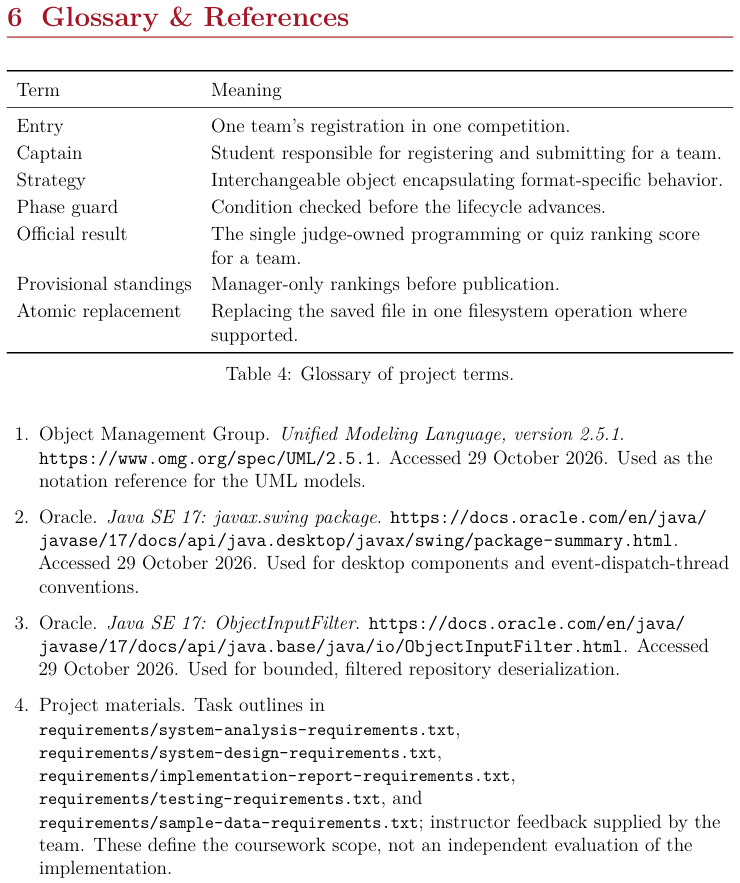
\includegraphics[width=\linewidth]{../assets/tables/06-glossary-references.png}
\clearpage\appendix
\section{Interface Mockups and Implemented Screens}
\subsection{Design Direction}
Wireframes and a clickable prototype guided our interface design. We built low-fidelity wireframes to sketch the layout and chose interface patterns suited to the application. We also built a high-fidelity clickable prototype to illustrate how a running program would behave. The clickable prototype and Java app share colors, fonts, and the overall design. A key difference is account access: the prototype has a role-switching control, while the Java app requires sign-in.
\subsection{Navigation and Role Paths}
\tableimage{05-navigation-paths}
\clearpage\subsection{Low-Fidelity Skeletons}
Editable SVG files are in \code{reports/assets/wireframes}. PNG previews are generated by \code{scripts/generate-wireframes.py}; they are schematic assets, not screenshots.
\screenpair{wireframes/01-overview.png}{Dashboard: featured call to action, metrics, and competition cards.}{wireframes/02-competition.png}{Competition workspace: persistent rules, stage strip, role action, and detail tabs.}
\clearpage
\subsubsection*{Evaluation and bracket views}
\screenpair{wireframes/03-judging.png}{Judging concept: review context alongside scoring fields. The implementation uses separate reader and scoring dialogs.}{wireframes/04-bracket.png}{Bracket concept: seeded opponents, next-round progression, and champion.}
\clearpage\subsection{Clickable Browser Prototype}
We built a prototype using HTML, CSS, and JavaScript to confirm the application's design. Instead of logging in, users switch roles with a button; the prototype already shows a signed-in workspace. Dates, locations, and event names are illustrative. It uses temporary sample data and does not connect to the Java application's saved data.
\screenpair{prototype/01-overview.png}{Browser prototype: overview and discovery cards.}{prototype/02-registration.png}{Browser prototype: project registration workspace.}
\clearpage
\subsubsection*{Scoring and knockout interactions}
\screenpair{prototype/03-scoring.png}{Browser prototype: live project weighted-score dialog.}{prototype/04-bracket.png}{Browser prototype: active knockout bracket.}
\clearpage\subsubsection*{Quiz and League Interactions}
\screenpair{prototype/05-quiz.png}{Browser prototype: official quiz points entry for each sample team.}{prototype/06-league.png}{Browser prototype: fixtures and league standings with a draw and completed results.}
\clearpage\subsubsection*{Creation Preview}
\begin{figure}[H]\centering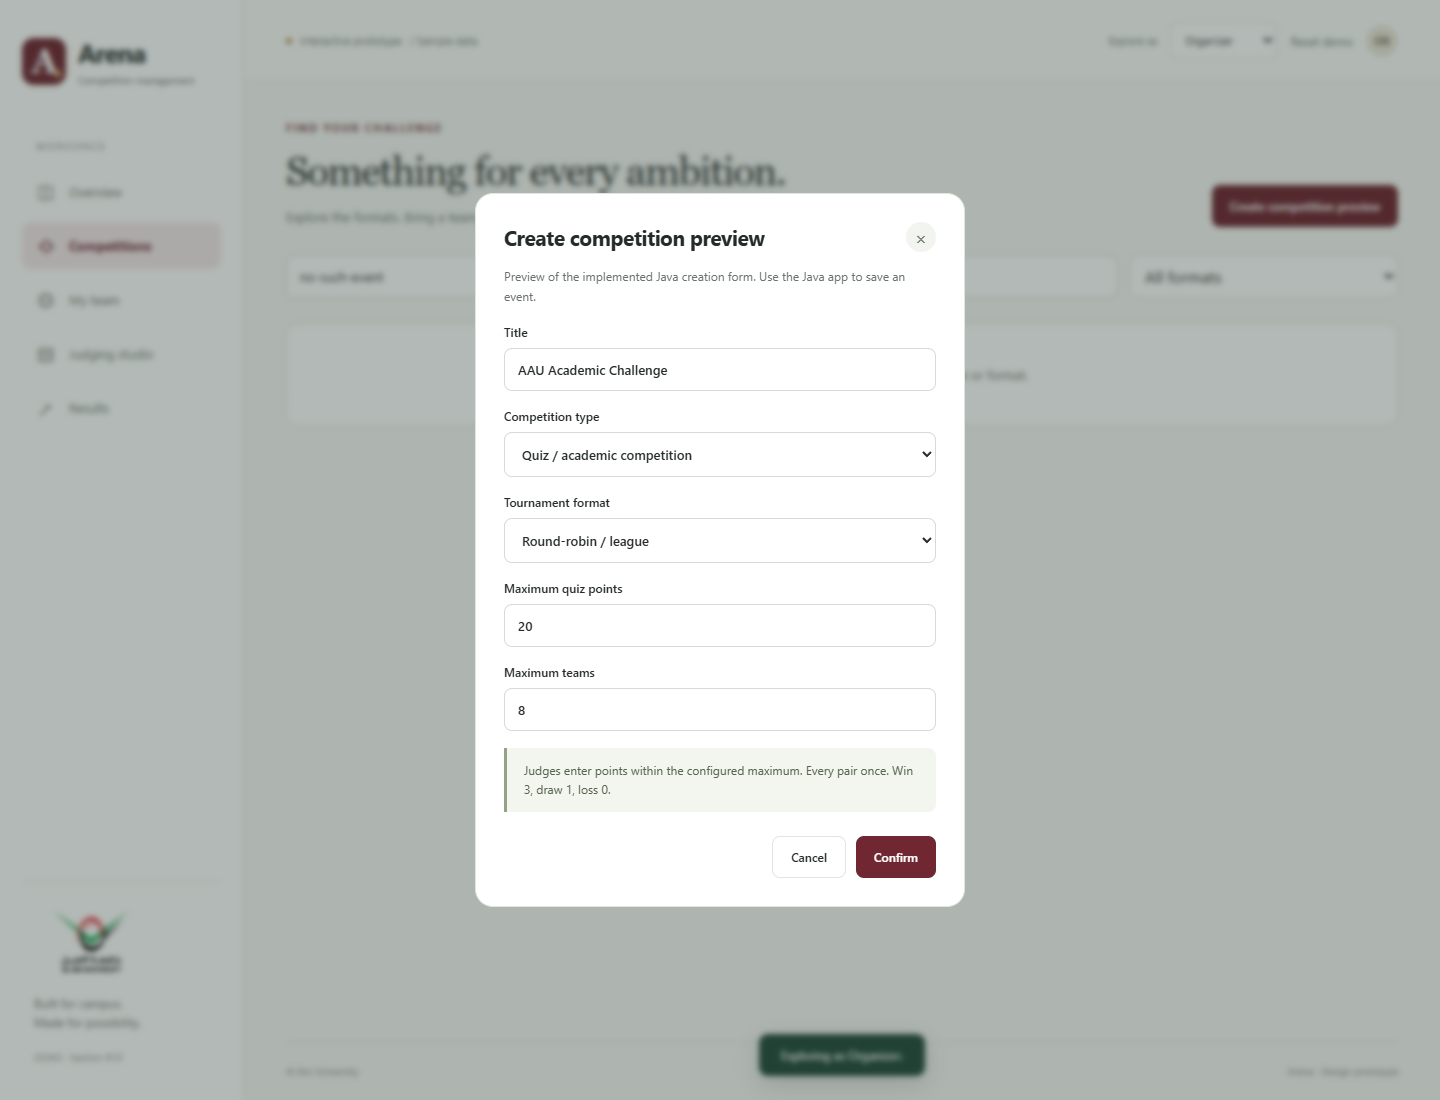
\includegraphics[width=0.90\linewidth,height=0.68\textheight,keepaspectratio]{../assets/prototype/07-creation.png}\caption{Browser creation preview filters formats by competition type. It explicitly directs actual saving to the Java application.}\end{figure}
\clearpage\subsection{Implemented Screens}
The following images were captured from actual Java Swing components at a 1440 by 1150 window size. These pictures show the interface layout; they do not, by themselves, test the application's behavior.
\screenpair{screenshots/01-sign-in.png}{Sign-in screen with a visible local demonstration account.}{screenshots/02-overview.png}{Organizer overview with competition and team metrics.}
\clearpage
\subsubsection*{Competition discovery and workspace}
\screenpair{screenshots/03-competitions.png}{Competition browsing with text search, format filter, and creation action.}{screenshots/04-competition.png}{Project-format workspace during registration.}
\clearpage
\subsubsection*{Bracket progression and published results}
\screenpair{screenshots/05-bracket.png}{Active robotics bracket with seeded semifinal matches.}{screenshots/06-results.png}{Published programming leaderboard with score and penalty details.}
\clearpage
\subsubsection*{Team directory and assigned judging}
\screenpair[0.26]{screenshots/07-teams.png}{Team directory with captain and roster details.}{screenshots/08-judging-studio.png}{Judging studio showing only the current judge's assigned competitions.}
\clearpage\subsubsection*{League Fixtures and Standings}
\screenpair{screenshots/09-league-fixtures.png}{Actual Swing league fixtures, selected-row scoring action, and publication policy.}{screenshots/12-league-table.png}{Actual manager-only provisional table with played, wins, draws, losses, scores, difference, and points.}
\clearpage\subsubsection*{Quiz and Match Scoring}
\screenpair{screenshots/11-quiz-score-dialog.png}{Actual quiz scoring dialog with a single relevant points field.}{screenshots/10-match-score-dialog.png}{Actual match-score dialog; league draws are allowed, while knockout draws are rejected.}
\clearpage\subsubsection*{Competition Creation}
\begin{figure}[H]\centering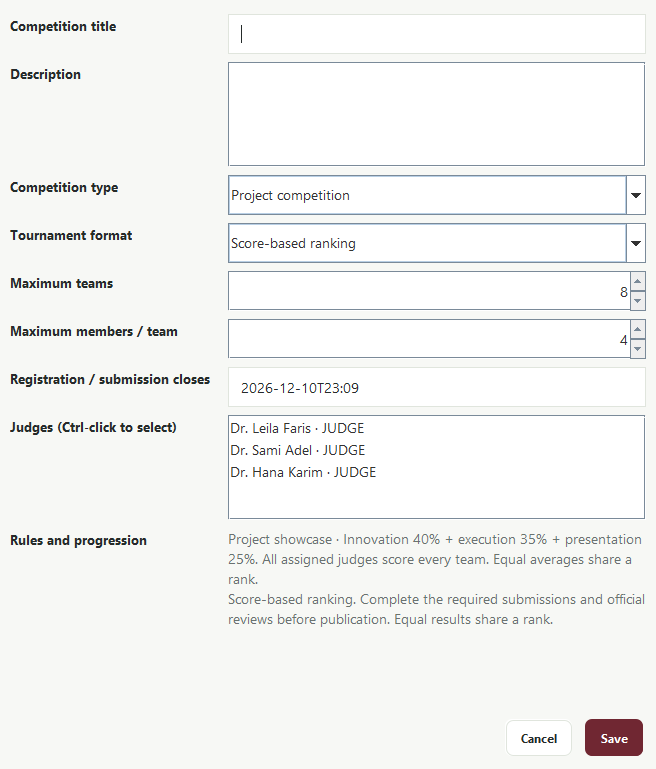
\includegraphics[width=0.90\linewidth,height=0.58\textheight,keepaspectratio]{../assets/screenshots/13-create-competition.png}\caption{Actual creation dialog with separate type and tournament selectors, relevant settings, assigned judges, and rule explanations.}\end{figure}
\subsection{Interaction States and Accessibility}
The interface should show when something is incomplete or unusual. An empty results view explains that publication is still pending. Missing selections prompt the user to choose a row. Invalid input displays a descriptive message and prevents the action from continuing. Tooltips reveal long values.

\subsection*{AI Assistance Disclosure}
We used an AI agent to generate and revise application code and documentation from the requirements, information, and feedback we supplied. This report includes wording revised by the team. AI assistance does not establish individual contributions; those must be confirmed by the group.
\end{document}
